\documentclass[sigconf]{acmart}

% remove copyright stuff for submission
\settopmatter{printacmref=false} % Removes citation information below abstract
\renewcommand\footnotetextcopyrightpermission[1]{} % removes footnote with conference information in first column
\pagestyle{plain} % removes running headers

\usepackage{comment}
\usepackage{tabularx}
\usepackage{pifont}
\usepackage{outlines}
\usepackage{graphicx}
\usepackage{minted}
\setminted{fontsize=\footnotesize,
breaklines}
\usepackage{caption}
\usepackage{subcaption}
\newcommand{\currentfontsize}{\fontsize{\f@size}{\f@baselineskip}\selectfont}
\setmintedinline{fontsize=\currentfontsize}



% minted: don't show red boxes around syntax errors in code
\AtBeginEnvironment{minted}{%
  \renewcommand{\fcolorbox}[4][]{#4}}

\usepackage[boxed,linesnumbered]{algorithm2e}
\SetAlFnt{\small}

\newcommand{\para}[1]{\smallskip\noindent{\bf #1}}
\newcommand{\allnotes}[1]{} 
\renewcommand{\allnotes}[1]{\textit{#1}}
\newcommand{\noteamy}[1]{\allnotes{\textcolor{violet}{[Amy: #1]}}}
\newcommand{\notesf}[1]{\allnotes{\textcolor{teal}{[SF: #1]}}}
\newcommand{\sr}[1]{\allnotes{\textcolor{blue}{[SR: #1]}}}
\newcommand{\notessm}[1]{\allnotes{\textcolor{red}{[SM: #1]}}}

\newcommand{\missing}[1]{\textcolor{purple}{#1}}

\newcommand{\sys}{Zed}
\newcommand{\zng}{ZNG}
\newcommand{\zst}{ZST}
\newcommand{\zson}{ZSON}

\newcommand{\tinydag}{\textsuperscript{\dag}}
\newcommand{\tinystar}{\textsuperscript{$\star$}}
\newcommand{\tinydiamond}{\textsuperscript{$\diamond$}}

% Compact itemize and enumerate.
\usepackage{enumitem}
\newenvironment{CompactItemize}
  {\begin{itemize}[noitemsep,topsep=0pt,leftmargin=*]}
  {\end{itemize}}
\newenvironment{CompactEnumerate}
  {\begin{enumerate}[noitemsep,topsep=0pt,leftmargin=*]}
  {\end{enumerate}}

\newcommand{\checkmark}{\textcolor{black}{\ding{51}}}
\newcommand{\xmark}{\textcolor{red}{\ding{55}}}
\newcommand{\nosupport}{\textcolor{black}{\ding{55}}}
%\usepackage[geometry]{ifsym}
%\newcommand{\optional}{\textcolor{black}{\Circle}}
%\newcommand{\optional}{\textcolor{black}{\ding{109}}}
\newcommand{\optional}{\textcolor{black}{\ding{55}}}

% macro for removing non-essential content in submission. used mostly
% for citations because references count towards the page limit.
% short form goes first, uncomment the second line to use long form
\newcommand{\shortorlongform}[2]{#1}
\renewcommand{\shortorlongform}[2]{#2}

\newcommand{\inlinefontsize}{\normalsize}

\begin{document}

\title{\sys{}: Leveraging Data Types to Process Eclectic Data}
\author{Amy Ousterhout\tinydag, Steve McCanne\tinystar, Henri Dubois-Ferrier\tinydiamond, \\Silvery Fu\tinydag, Sylvia Ratnasamy\tinydag, Noah Treuhaft\tinystar}
\affiliation{\institution{UC Berkeley\tinydag \quad \quad Brim Data\tinystar \quad \quad 12\textsuperscript{th} Ave Labs\tinydiamond}}

\begin{abstract}
    
Data-processing systems increasingly face data that is {\em eclectic}---it spans many heterogeneous schemas and its schemas evolve over time. 
Unfortunately, existing approaches for processing and querying data are not ideal for eclectic data since they impose a tradeoff between efficient querying and simplicity. 
We argue that this limitation stems from the very foundations of data processing: data models and their corresponding query languages. No existing approach---whether relational, document, or hybrid---is designed to enable ingesting, querying, and reasoning about heterogeneous types of data. In this paper we propose \sys{}, a new approach to data processing that centers around {\em data types}. \sys{} elevates data types to be first-class members of both the data model and query language, and by doing so offers a promising path towards easing the processing of eclectic data.
    
\end{abstract}




%Unfortunately, no existing approach for processing and querying data is ideal for eclectic data. Existing systems enable either efficient querying and introspection of homogeneous data (as in relational databases), or the ability to flexibly accommodate heterogeneous data (as in document stores), but not both at the same time for the same data. Even recent hybrid systems that aim to unify the document and relational approaches fail to provide the best features of both at the same time for the same data. 

\maketitle
\pagestyle{plain}

\vspace{-1em}
\section{Introduction}

The nature of data is changing, driven by growing applications such as IoT and monitoring as well as an increasing desire to relate data that spans multiple administrative domains. As a result, data today is {\em heterogeneous}---it spans many different schemas---and {\em evolving}---its schemas change frequently and sometimes unexpectedly. This data with diverse and dynamic schemas---that is, {\em eclectic data}---raises new challenges with ingesting, storing, and querying data. 
In particular, with eclectic data, the process of data discovery becomes a crucial part of the processing pipeline. When data does not conform to a small and well-known set of schemas, then the first step to processing the data is to understand the ``structure’’ of a given data set: discovering what schemas are present, how often each occurs, how similar or dissimilar particular schemas are, and so forth. We use the term {\em data introspection} to refer to this process of exploring the structure of a dataset. Only once users understand the structure of their data can they take steps to transform, clean, or otherwise ``prepare’’ the data for additional processing. In total these steps —  spanning introspection and preparation — can be extremely time consuming, taking 80\% or more of analysts' time~\cite{civilizer}. 

The databases community has long recognized this shift toward eclectic data and, over the last two decades, has vigorously debated different approaches to representing and processing diverse data~\shortorlongform{\cite{what_goes_around, redbook}}{\cite{what_goes_around, redbook_intro}}. Today, the community has largely converged on two data models, which are known to have different strengths and weaknesses. The {\em relational model's} rigid structuring of data according to explicit schemas~\shortorlongform{}{\cite{codd_data_banks, codd_1990}} enables efficient querying and formats such as columnar~\shortorlongform{\cite{dremel, cstore}}{\cite{dremel, cstore, column_vs_row}} as well as data introspection~\cite{aurum}.
%\sr{don't we want to say that the need for sophisticated data introspection and preparation is greatly diminished in this model? if so, move ref to aurum elsewhere}\noteamy{I agree that it's diminished, but at some point we need to say that introspection is easy in the relational model, in order to set up that part of the catch-22}. 
It is the model of choice for analytics in relational databases\shortorlongform{}{~\cite{postgres, sqlite, sql_server, oracle}} and nested variants of it form the foundation of big data systems~\cite{avro, parquet, dremel, spark, delta_lake}. However, ingesting eclectic data is challenging in the relational model. On the other hand, the {\em document model's} self-describing data values make it trivial to mix heterogeneous data and to ingest data with never-before-seen schemas. Thus data sources commonly generate data in the document model (e.g., JSON), and document databases leverage this model to enable easy ingestion and querying of eclectic data~\cite{mongo, couchbase}. However, this approach sacrifices efficiency and clarity about what kind of data is present. 

It is well-recognized that neither the relational nor document model is always best.
%with each of the relational and document models providing functionality that the other lacks.
As a result, several recent research efforts and industrial deployments attempt to combine these two and achieve the best of both. For example, some approaches such as AsterixDB can be configured to behave like either the relational model or the document model~\cite{asterixdb, sql++}, while others such as Snowflake or Lakehouses can store some data in each model~\cite{snowflake, postgres, bigdawg, dbms+, delta_lake, lakehouse}.

Unfortunately, as we will discuss (\S\ref{s:hybrid}), even these combined approaches are far from ideal. First, users must contend with two data models: they must decide how to split or replicate their data across both models and a single query can typically leverage the benefits of only one model. Second, to achieve the benefits of explicit schemas, users still have to clean their data from the document into the relational model. This cleaning process is known to be complex and brittle~\shortorlongform{\cite{civilizer}}{\cite{civilizer, databricks_json_data_ingest}}, especially without effective introspection tools to discover what kinds of data are present in the first place. And yet, thirdly, these systems do not make introspection over document data any easier. Thus users are stuck in a catch-22: in order to clean data they must be able to introspect over it, yet in today's systems, rich introspection is only possible after the data has been cleaned.

We believe that these approaches fall short because they are {\em hybrid} rather than truly {\em unified}. They co-implement both models,
%and require a shim layer on top. This is complex and brittle,
but a given piece of data can only benefit from one model at a time.
Taking a step back, we wondered if this sacrifice is truly necessary, or if a solution could be found by addressing the problem at a lower layer. Perhaps it is time, yet again, to rethink the foundations of data processing: the data model and its corresponding query language.
We argue that eclectic data would benefit from a {\em new approach to unification} in which a single data model can simultaneously provide the benefits of both explicit schemas (efficient analytics, ease of introspection) and mixed heterogeneous data (seamless ingestion, query results that span heterogeneous data).% In addition, this model must provide comprehensive support for data introspection.


\begin{figure*}[t]
    \centering
    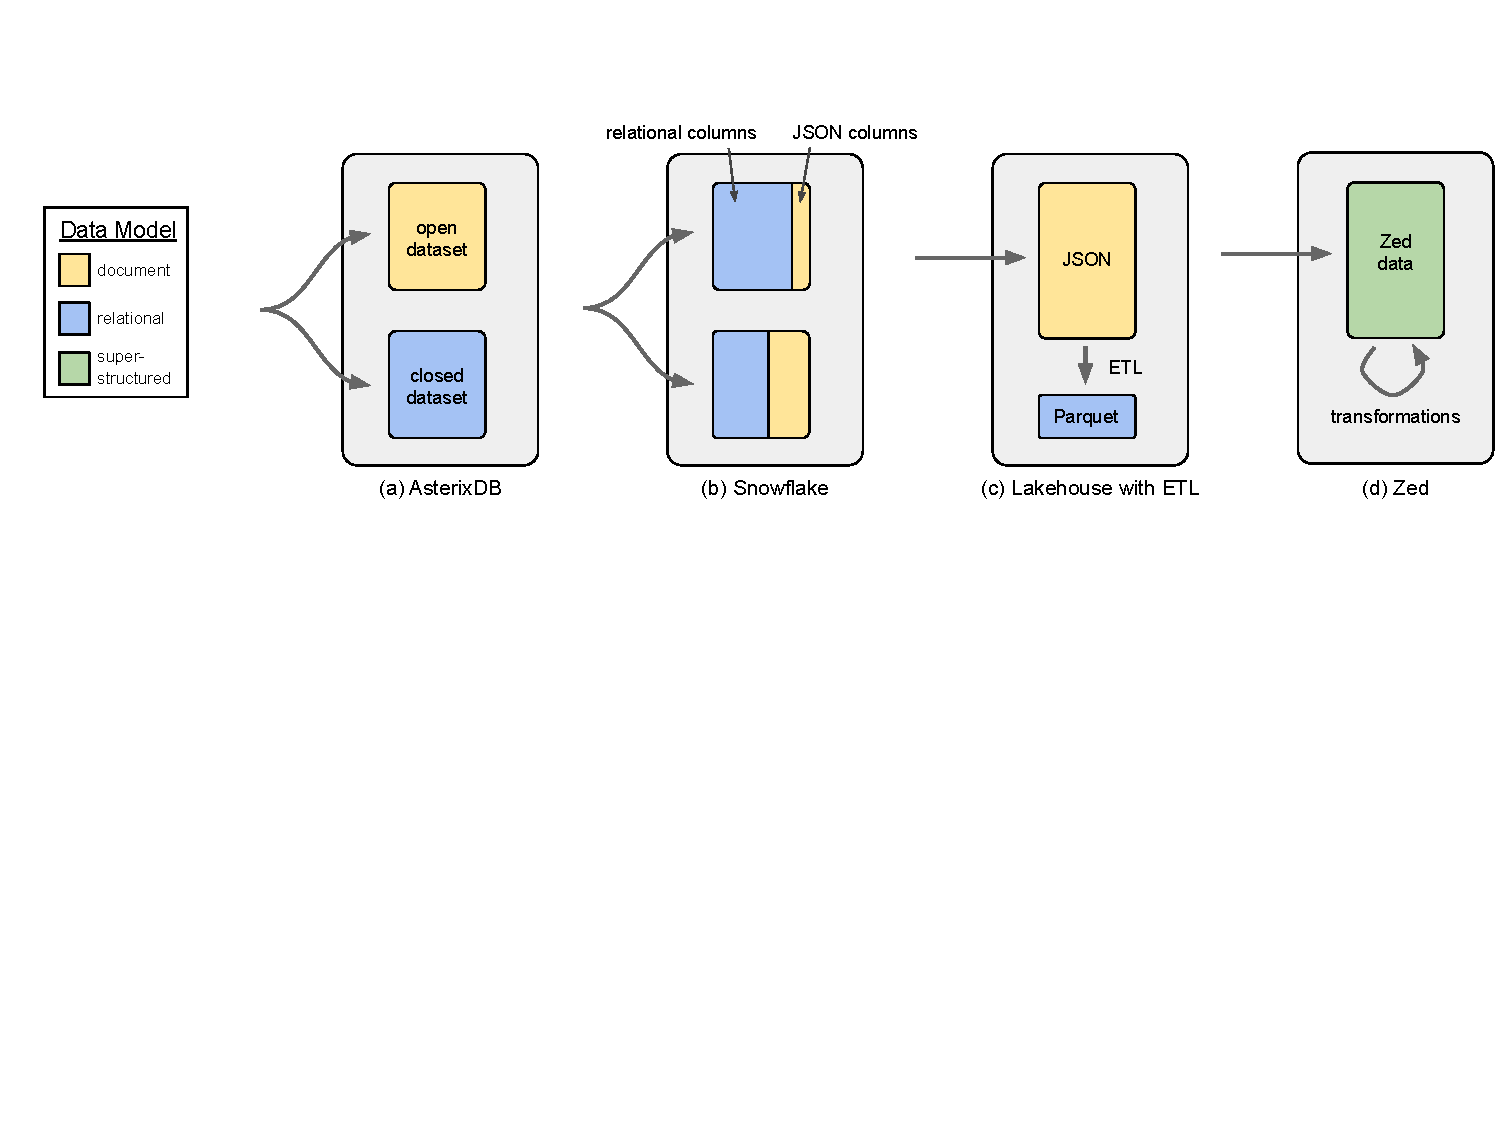
\includegraphics[width=0.81\textwidth]{figures/hybrid_approaches.pdf}
    \vspace{-1.3em}
    \caption{Three example hybrid approaches to data processing: (a) AsterixDB splits incoming data into open and closed datasets in separate files, (b) Snowflake adds columns of JSON data to each relational table, and (c) Lakehouses use ETL to clean a subset of JSON data into Parquet. (d) In Zed, all data (raw or transformed) is represented in the super-structured data model.}
    \label{f:hybrid_approaches}
    \vspace{-1.6em}
\end{figure*}

We start with the observation that what fundamentally enables both efficient analytics and data introspection is knowing the {\em type} of each piece of data. For example, this allows us to store data in formats that are organized by type (e.g., by column) and to query for information about what types of data are present. The relational model has this explicit type information, but is overly rigid in how it uses it, only accepting data from a pre-defined set of schemas. 
Unfortunately, attempts to relax this rigidity have often introduced new problems. For example, some add new external components (e.g., schema registries~\cite{confluent_schema_registry}) that must be integrated with the data processing pipeline, while others incorporate partially typed data (e.g., Snowflake's \texttt{OBJECT} type~\cite{snowflake}) and thus lose some of the benefits of type information.
This leads us to the goal of defining a data model in which every data value has an explicit type and yet there are no constraints on which types are permitted to coexist (e.g., in the same file, table, or set of query results). In other words, our goal is {\em comprehensive yet flexible typing}.
%In addition, this type information must be queryable, by which we mean that users can query {\em by} type (e.g., returning all data of a specified type), or \emph{for} type (e.g., returning what types exist in the data set). As we'll see, making types queryable is key to enabling rich data introspection. \noteamy{can we cut the previous 2 sentences? covered by the query language paragraph below}
In addition, this data and its type information should be self-contained so that parsing data never requires coordination with an external registry; instead users can query both data and types in a single unified manner. 

%\sr{Needs some connecting tissue here to lead the reader to types as the answer? Can we say something like: We start with the observation that what fundamentally enables both efficient analytics and data introspection is knowing the \emph{type} of data we have. Having type information allows us to, for example, use formats that organize data by type (e.g., by column) for efficent processing, and allows us to reason about the shape of data available (e.g., how many types exist, how many records of each type). The relational model has the well-defined type information that we seek but the problem is it’s overly rigid in its use of this type information — only accepting data from a pre-defined set of types. And attempts to relax this rigidity have introduced new problems — e.g., they add new external components (e.g., schema registries) that require complex integrations with the storage and query processing components, or they resort to weakly defined types (e.g., object) that can’t fully utilize the benefits of types. This leads us to the goal of defining a data model in which all data is typed but that doesn’t constrain what types are permitted. Moreover, this data together with its type information should be self-contained - i.e., the data model must capture both data and their type information in one coherent architecture. These observations lead us to a new data model in which \ldots.} 
%Our unified approach begins with two goals, centered around {\em data types}. First, every data value should have an explicit, queryable type. This enables efficient storage and querying, avoids error-prone schema inference, and enables queries about data types, such as introspection and shaping. At the same time, we should be flexible about which data types are allowed to coexist in the same file, table, or set of query results.
%\noteamy{need to rework the previous 2 paragraphs. they focus too much on limitation 1 and don't really cover 2 or 3.}

%\notesf{I don't find the key idea come through crisply from the current text in the two paragraphs below and I think we should mention schema registries. Let's discuss?}

The key to achieving comprehensive yet flexible typing is to change the way that we associate type information with data values. Instead of associating a single schema with each file or table, which makes it difficult to store or process heterogeneous data together, we propose a new {\em data type abstraction} that is associated directly with individual data values. This enables each value to have an explicit data type (as in the relational model) but also allows different values that are processed together to have different types (as in the document model). We call the resulting data model the {\bf super-structured data model}, because it subsumes the structures of the relational and document data models. Data is organized as a sequence of typed values; when all values have the same type, this model is equivalent to the relational model.

%\sr{Elaborate? I.e., data is ingested as an ordered stream of typed values. And when all data are the same type, the super-structured model is equivalent to the relational model}\notesf{I strongly agree; I find this a key observation.} 

% \notesf{summarize this by saying ``deep typing without schema rigidity''?} \noteamy{I'm not sure that ``deep typing without schema rigidity'' quite captures the key properties of \sys{}. If we want a summary at that level of detail, what about: ``type flexibility and first-class types''?}

Realizing this approach requires care in designing the type abstraction. We propose an abstraction with the following properties:
\begin{CompactItemize}
    \item Types are {\em associated with individual values}, rather than with a collection such as a table or file.
    \item Types are {\em complete} - we observe that catch-all types such as \texttt{OBJECT} or \texttt{JSON}, or allowing a value to include extra fields beyond those specified by its type prevent the full benefits of types.
    \item Types are {\em first class} - users can query for data types and the query results---which contains types---are returned in the same data model. Users can refer to types by name and data formats can assign numeric type IDs for efficient storage and querying.
    %\item Data types should be {\em identifiable} (i.e., types can be referred to by a numeric ID or string name) - this enables efficient storage and querying because data values can be tagged with their numeric type. It also enables querying values by their type, e.g., to extract all values with a given type, effectively extracting a single relational table from heterogeneous data.
    \item Type definitions are {\em inlined} - this enables data sources to define new types on the fly without out-of-band coordination or additional burden relative to writing JSON data.
\end{CompactItemize}

However, a new data model alone cannot provide the introspection and unification that we seek; we also require a corresponding query language that can exploit the full power of this data model. While the data model encodes per-value type information, the role of the query language is to expose this type information to users. Users should be able to query {\em by} type (e.g., returning all data of a specified type), or \emph{for} type (e.g., returning the type of a data value).
%query {\em for} the type of each individual data value, and to query data values {\em by} type.
In short, types must be {\em first-class members} of the query language as well. This enables rich introspection and is crucial for truly subsuming both the document and relational models. Querying by type allows a user to extract all values with a given schema; the returned data corresponds to a table in the relational model and can be processed as such.



\begin{comment}
\sr{todo. Text that says} 
Data model is only half the story. The other is that we need a corresponding query language that exploits the power of the data model. In our case, this means supporting types as a first-class primitive in the query language - query by type, query for type, operators (compare etc) over types. 
Thus our query language is designed to leverage and complement the properties of the data model: that type information is associated with data, and that this type information is inline with the data (self-contained). 
This enables data introspection. But also allows us to realize the promise that a super-structured data model subsumes both relational and document models. E.g., query by type allows us to extract all records that conform to a particular schema; the returned records correspond to a table in the relational model and can be processed as such.
\end{comment}

In this paper we propose {\bf \sys{}}, a new approach to data processing that is centered around these data types. \sys{} includes a new super-structured data model (\S\ref{ss:zed_data_model}) and query language (\S\ref{ss:zed_query_language}). In addition, \sys{}'s type abstraction allows data to be represented in the format most suitable for the task at hand: columnar for analytics, human-readable for debugging, etc.  Because all data is typed, converting it between formats within the family is lossless and fully automated. Thus \sys{} includes a ``family of data formats'' (\S\ref{ss:zed_formats}). Finally, we will show how \sys{} overcomes the challenges of existing hybrid approaches and unifies the document and relational models in a new way, {\em embodying both at the same time}  (\S\ref{s:zed_in_action}). %\sys{} enables: easy data generation and ingestion, with the ability to create new types on the fly; efficient storage and analytics; data introspection at any stage of data processing; and simplicity, with no dependency on external components such as schema registries (\S\ref{s:zed_in_action}).

%\vspace{-1em}

\section{The Limitations of Hybrid} \label{s:hybrid}

As pointed out by prior work, the relational model's rigid schemas and the document model's lack of schemas each create significant challenges for users~\cite{snowflake, lorel, asterixdb, what_goes_around}. {\em Hybrid} approaches have emerged in response, attempting to combine the two models to achieve the best of both.\shortorlongform{}{\footnote{Note that when we refer to ``hybrid systems,'' we refer to the subset of ``multi-model systems''~\cite{multi_model} that relates to the relational and document data models.}} There are many such hybrid systems, including research approaches~\cite{asterixdb, sql++, bigdawg, dbms+} and industry examples~\cite{postgres, snowflake, lakehouse, delta_lake, partiql}. These approaches can simplify multi-model deployments, but no consensus has emerged regarding which is best, and each still faces significant challenges.

In this section, we illustrate the limitations of hybrid systems during ingestion (\S\ref{ss:hybrid_ingestion}), querying (\S\ref{ss:hybrid_querying}), and data introspection (\S\ref{ss:hybrid_schema}). For the sake of concreteness, we focus on three specific systems; other hybrid systems often face similar limitations.
Figure~\ref{f:hybrid_approaches} shows the three example systems and configurations.

\para{AsterixDB~\cite{asterixdb}.} AsterixDB's data model is a superset of JSON that also includes a schema language. It supports both ``open Datasets'' of heterogeneous document-model data and relational-like ``closed Datasets'' of homogeneous data. All data can be queried with AsterixDB's AQL or with SQL++~\cite{sql++}. In our example configuration, data with known schema is validated and stored in ``closed Datasets'' while the rest is stored in ``open Datasets''.

\para{Snowflake~\cite{snowflake}.} Snowflake extends traditional relational data warehouses with support for semi-structured data. This is done primarily via columns of type \texttt{OBJECT} that can store JSON documents, as well as corresponding extensions to SQL.\footnote{MySQL\shortorlongform{}{~\cite{json_type_mysql}} and PostgreSQL\shortorlongform{}{~\cite{json_type_postgres}} offer similar functionality with a \texttt{JSON} type.} In our configuration, all data is stored in Snowflake tables, with the heterogeneous, nested, and dynamic portions stored in such columns of JSON.

\para{Lakehouse with ETL~\cite{delta_lake, lakehouse}.} Lakehouses store all data (whether raw or processed) in a data lake and query it using SQL or dedicated libraries. In our configuration, all incoming data is stored directly in the lake and ETL is used to clean a subset of the data into Parquet files~\cite{parquet} for efficient analytics.\footnote{Parquet's data model is the relational model, extended to support nested data.}

\vspace{-0.7em}
\subsection{Data Ingestion} \label{ss:hybrid_ingestion}

Data sources today often generate data in a schemaless format such as JSON~\cite{json}. Users choose JSON over alternatives such as Avro~\cite{avro} or Protocol Buffers~\cite{protobufs} because it enables heterogeneous data to coexist in a file and it avoids the upfront complexity of defining and agreeing on schemas. When JSON data arrives at a storage layer for ingestion, hybrid approaches face two main challenges.

\para{Cleaning data into the relational model.} In order for data to fully benefit from schemas (for data introspection and efficient queries and storage), it must be converted from JSON into the relational model. The challenges of this are well-known: data must be matched to and validated against the relevant schema and any non-conforming data must be cleaned or dropped\shortorlongform{}{~\cite{databricks_json_data_ingest}}. Automated approaches to this such as Fivetran\shortorlongform{}{~\cite{fivetran}} or Informatica\shortorlongform{}{~\cite{informatica}} can be error-prone and brittle in the face of changing schemas.
%, and they encapsulate ingestion complexity rather than eliminating it.
This problem first arose with purely relational systems, and because hybrid systems store some data in the relational model, they suffer from it as well.

\para{Which model for which data?} Users of hybrid systems face the challenge of deciding which data model to use for which parts of their data. Users of AsterixDB must decide which Datatypes are stable enough to be able to leverage closed Datasets; users of Snowflake must decide which fields of their data are eclectic enough to warrant \texttt{JSON} columns and when data is different enough to warrant a separate table altogether; and users of Lakehouses must decide which data to ETL into Parquet. These decisions impact how users will be able to query their data (\S\ref{ss:hybrid_querying}), and
%how efficient those query executions will be. Furthermore,
if users want to convert data between models later, they may encounter the challenges and delays of cleaning their data, as described above.

\vspace{-0.8em}
\subsection{Querying Data} \label{ss:hybrid_querying}

Different data models provide different benefits during querying. However, in hybrid approaches, most data is only stored in one model or the other; this is the case for all data in our AsterixDB and Snowflake configurations, and the JSON data that isn't ETLed into Parquet in the Lakehouse. This data can typically only benefit from the properties of the data model that it is stored in.

For example, the relational model's schemas enable introspection queries that explore what kinds of data are present~\cite{aurum} and high-performance querying over efficient formats~\cite{snowflake, parquet, dremel, cstore}. For data stored only in the document model, these benefits are not available.
%This applies to data stored in open Datasets in AsterixDB, JSON columns in Snowflake, or JSON in the Lakehouse.
A rich body of literature attempts to infer schemas over this kind of data\shortorlongform{~\cite{parametric_schema_inference, schema_management, adaptive, liu2016closing, snowflake, asterixdb_compaction}}{~\cite{parametric_schema_inference, discala2016automatic, schema_management, bex2006inference, adaptive, liu2016closing, deriving_rdf_schema, snowflake, asterixdb_compaction, drill, baazizi2017counting, schema_inference_json, liu2015management}} but these heuristics can be inaccurate.\footnote{Schema inference over data in property graphs or RDF faces similar challenges~\cite{deriving_rdf_schema, neo4j}.} For example, human intervention may be necessary to determine whether two values have the same or different schemas in document-model data in AsterixDB or the Lakehouse.

On the other hand, the document model enables queries that can flexibly mix heterogeneous data~\cite{lorel, asterixdb}. For example, consider a query to sort all data by time and return the five earliest records, effectively: \texttt{SELECT * FROM * ORDER BY time LIMIT 5}. This query is straightforward to issue over JSON data, even if the data and results span multiple schemas. However, to issue this query over relational data, the user must first combine heterogeneous tables into a wide ``uber table'' whose ``uber schema'' contains the union of all columns spanned by the data. The results for this query are then presented as a very wide table, bloated with many \texttt{null} values. Notably, AsterixDB does not suffer from this problem. Even though data in a closed Dataset is by definition homogeneous, AsterixDB's data model is a superset of JSON, and AsterixDB query results can mix heterogeneous data, similar to JSON. In contrast, issuing this query across Snowflake tables with differing relational columns will trigger the same problem as in purely relational systems.

%If the user issues this query over the JSON data, they can sort the logs and return the first 5, but will have no notion of the schema of each. If the user attempts to issue this query over the Parquet data, they must first combine the heterogeneous logs into a wide table whose ``uber schema'' contains the union of all columns spanned by the logs. However, this ``uber table'' lacks information about the original schema of each log, preventing the analyst from obtaining the schemas of the first 5 logs. This query cannot be issued in existing systems today---even hybrid systems---because displaying the results requires both schema information and the ability to mix heterogeneous records, which are not possible within a single existing data model.

\vspace{-1em}

\subsection{Data Introspection} \label{ss:hybrid_schema}

With the rise of eclectic data, users are increasingly interested in {\em data introspection}. Users want to query data {\em for its schema}, for example to enumerate the schemas spanned by a dataset and how many records have each. Users also want to query data {\em by its schema} to select a subset of data with particular schemas for further exploration. 
%for example to extract the equivalent of a relational table out of a stream of heterogeneous data.
%and {\em shaping} enables users to transform data from one schema to another.
Users may want to perform these tasks at any stage of processing: during ingestion, on stored data, or over query results.

The relational model does enable some forms of data introspection. For example, users can query \texttt{INFORMATION\_SCHEMA} to list tables and their column names and types, or query external systems like Aurum~\cite{aurum}.
%To shape relational data, users can use statements like \texttt{ALTER TABLE} or systems such as PRISM~\cite{prism}, CoDEL~\cite{codel}, or BiDEL~\cite{bidel}.
However, the relational model and query languages for it lack support for referring to schemas holistically. Some query languages such as N1QL enable users to query by or for field types (e.g., with \texttt{ISSTRING()} or \texttt{TYPE()} functions), but these only work for primitive types and return ``object'' or ``json'' for more complex data~\cite{sqlite, n1ql, mongo}. As a result, the relational model does not support queries by schema, because it can neither mix heterogeneous data together nor refer to schemas in queries. Introspection in the document model is even more challenging, because it lacks explicit schemas. In addition, inferring the schema of data or which data has the same schema can be inaccurate and brittle (\S\ref{ss:hybrid_querying}).

%In addition, introspection and shaping must be performed field-by-field; there is no way to express the entire schema of a table as a single value in query results or to succinctly express shaping rules such as ``drop all columns from table A that are not present in table B.''\footnote{Note that some prior work enables queries or query results to refer to table names or database names~\cite{relation_names, fisql_2005, fisql_2007, schemasql}, but not an entire schema.}

%Finally, languages developed for hybrid systems can query data in both the document and relational models, but do not make it any easier to manipulate data by its schema. For example, neither the query languages supported by AsterixDB (AQL~\cite{asterixdb} and SQL++~\cite{sql++}) nor Snowflake's SQL extensions~\cite{snowflake} provide a holistic way to refer to schemas in queries or in query results.

Unfortunately, this puts users in a catch-22. In order to clean their data into the relational model, users need to first understand what kinds of data are present, but the limited tools for introspection that are available today are only available for data in the relational model. In short, it is difficult for users to introspect or clean their data until {\em after} it has already been cleaned into a pre-defined set of schemas. Furthermore, query languages for hybrid systems~\cite{asterixdb, sql++, snowflake, partiql}
%(e.g., AQL~\cite{asterixdb}, SQL++~\cite{sql++}, or Snowflake's SQL extensions~\cite{snowflake}) 
do not avoid this catch-22 because they do not provide a holistic way to refer to schemas in queries or in query results.
\vspace{-0.8em}
\section{The Design of \sys{}}

\sys{}'s key goal is to provide {\em fine-grained and flexible typing} throughout data processing. Achieving this goal allows \sys{} to unify the document and relational models 
%(embodying the best features of both simultaneously) 
and enable new functionality for data introspection. \sys{}'s key technique is a new {\em data type abstraction} that represents the structure of an individual data value; achieving fine-grained yet flexible typing is a new approach. We now describe \sys{} types and how they impact \sys{}'s data model (\S\ref{ss:zed_data_model}), %runtime (\S\ref{ss:zed_type_contexts}),
query language (\S\ref{ss:zed_query_language}), and formats  (\S\ref{ss:zed_formats}).

%A type in \sys{} plays a similar role as a schema of a row in a relational database or the implied type of a single JSON document. 

\begin{comment}
Realizing this type abstraction requires answering several design questions, such as:
\begin{CompactItemize}
    \item Type definitions - what should a type definition specify?
    \item Type evolution - how can we enable users to easily create new types on the fly?
    \item Type scope - what is the scope of a type definition and how can we relate types across different scopes?
    \item Querying types - how can we represent types in queries and in query results?
\end{CompactItemize}

In this section, we answer these questions by overviewing \sys{}'s super-structured data model (\S\ref{ss:zed_data_model}) and query language (\S\ref{ss:zed_query_language}). In addition, we observe that a single unified data model does not necessitate a single unified data format. As pointed out by prior work, no single format is best for all use cases~\cite{one_size_fits_all_2005, one_size_fits_all_2007}, and we describe how \sys{} supports multiple formats (human-readable, columnar binary, etc.) with lossless transformations between them (\S\ref{ss:zed_formats}). Finally, we explain how \sys{} manages type scope (\S\ref{ss:zed_type_contexts}).
\end{comment}

\vspace{-1em}
\subsection{\sys{} Data Model} \label{ss:zed_data_model}

\begin{comment}
The \sys{} data model is guided by two key principles. First:

{\bf P1:} {\em Every data value should have an explicit, queryable data type.}

\noindent{}{\em Explicit} types are an essential property of the relational model. They enable efficient storage formats~\cite{parquet, orc, protobufs, avro, dremel} and faster parsing and querying than with JSON data, which is known to be difficult to parse efficiently~\cite{mison, sparser}. Types that are also {\em queryable} enable rich data introspection, queries by type, and shaping by type (\S\ref{ss:hybrid_schema}). At the same time:

{\bf P2:} {\em We should be flexible about which data types are allowed to coexist in the same file, table, or query results.}

\noindent{}This {\em flexibility} is essential to the document model and allows any data value with valid syntax to be appended to a file, regardless of what other data or data types are already present in that file. This makes it easy to accommodate heterogeneous and evolving data without predefining its schema.
\end{comment}

We first describe the \sys{} data model and then highlight some of the unconventional design decisions behind it.

\subsubsection{Data Model}

The \sys{} data model consists of an ordered sequence of typed data values. Each value's type is either a primitive type (int32, string, bool, type, etc.), a complex type (record, array, set, map, union, etc.), a named type, or the null type. All of these types have analogs in other data models, and we describe the significance of some of them below. For example, consider \sys{} records. A record consists of an ordered set of named values called ``fields''. Field names are simply strings and field values can be any \sys{} value, with the types described above. This enables nested data, as a record can contain arrays, sets, other records, etc. A row in a relational table, a record in Avro, or a JSON document could each be represented using a single \sys{} record.

For example, consider the following two records of IoT sensor data, represented in \sys{}'s text-based format, ZSON, which supports native epoch 64-bit nanosecond times in ISO format:

\noindent{}\mintinline[fontsize=\inlinefontsize]{bash}{{ts:2022-09-01T00:00:00Z,temp:68(int32)}}

\noindent{}\mintinline[fontsize=\inlinefontsize]{bash}{{ts:2022-09-01T10:12:00Z,temp:68.(float32)}}

\noindent{}The first record has type \texttt{\{ts:time,temp:int32\}} while the second record has type \texttt{\{ts:time, percent\_humidity:float32\}}.
Despite having different types, these two records can be stored in the same file because data types in \sys{} are {\bf associated with individual data values}.

%Thus, a sequence of \sys{} records can be used to represent either homogeneous data, as in a relational table or Parquet file, or heterogeneous data, as in the document model.

Types are {\bf first-class members} of the \sys{} data model. This means that a type---even the type of a record---is a single entity, which can be represented as a \sys{} value whose type is {\em type}. As a result, a query for the type of a record returns the record's type in the same \sys{} data model, rather than a separate data model as in existing systems~\cite{aurum}. \sys{} also enables users to define {\em named types}, which bind a name to a type. For example, the ZSON includes decorator syntax for defining named types, e.g., \texttt{(=temperature)} to define a named \texttt{temperature} type:

\noindent{}\mintinline[fontsize=\inlinefontsize]{bash}{{ts:2022-09-01T00:00:00Z,temp:68(int32)}(=temperature)}

\noindent{}The \sys{} query language (\S\ref{ss:zed_query_language}) uses angle brackets to specify type values, thereby allowing users to refer to the type \texttt{\{time:time,temp:int32\}} using \texttt{<temperature>} in queries . For example, a query can extract all records with type \texttt{<temperature>}, the equivalent of a single relational \texttt{temperature} table.
%\sys{}'s binary data formats also leverage numeric type IDs for efficient encoding and querying (\S\ref{ss:zed_formats}).

%For example, a query for the type of the first record in Figure~\ref{f:iot_data} returns \texttt{<temp\_schema=\{time:time,temp:int32\}>}, and this result is still represented in the \sys{} data model.

Note that the data itself is defining the named types requiring the query engine to understand that a named type binding can evolve over time as data is processed.  When multiple bindings for a given type name conflict with one another, the system automatically converts the conflicting types into a named sum type, represented in \sys{} by a named union type of the underlying unique types encountered.  As long as various type operators in the query language support variations of type equivalence under this model, then powerful type-based introspection becomes possible. 

Type definitions in \sys{} are stored {\bf inline} with the data. When a new type first appears in a \sys{} file, the type definition is stored inline at that point in the file. The \texttt{temperature} record above shows how \sys{} does this in its text-based format; we describe  how \sys{} efficiently encodes type definitions in its binary formats in~\shortorlongform{\S\ref{ss:zed_formats}}{Section~\ref{ss:zed_formats}}. A consequence of inlined types is that type definitions are locally scoped, which means that values from different locally scoped type contexts must somehow be merged so that types from different contexts can coexist and be reliably compared. To do so, we carefully designed the \sys{} type system to allow merging of types to be implemented with a simple table lookup as described in Section~\ref{ss:zed_type_contexts}.

Finally, as with Parquet and Arrow, each type in \sys{} specifies the {\bf complete} and potentially nested structure of data values with that type. This contrasts with the document model, which provides only partial type information such as \texttt{OBJECT}, \texttt{JSON}, or \texttt{any}. In \sys{}, any value is nullable, e.g., a record of type \texttt{T} can omit fields of \texttt{T} by explicitly setting them to \texttt{null}; this avoids an combinatoric explosion in the number of defined types when different records omit different combinations of fields. Types are ``closed,'' meaning that a record of type \texttt{T} never contains extra fields beyond those defined by \texttt{T}.  That said, it is often useful to define the non-nullability of fields as a useful data constraint, but our philosphy is to defer such constraint enforcement to additional semantic layers above the \sys{} serialization layer, e.g., in an ingest pipeline or in a query language.

Complete types may appear to be at odds with \sys{}'s goal of flexibility. For example, suppose a temperature sensor outputs \texttt{temperature} records with two fields at first, but then adds a third \texttt{unit} field~\shortorlongform{}{ to \texttt{temperature}} so that it can output data as either Fahrenheit or Celsius, as shown in Figure~\ref{f:iot_data}, which is the classic "schema evolution" problem.  But as described above, in \sys{}, this simply implies a sum type of the variations encountered, which provides extreme flexibility in handling dynamically evolving eclectic data.  In this approach, the sum-typed data can simply flow through a query or into the storage layer unhindered, or the condition could be detected by ingest logic and the sum-types converted to a desired target type with \sys{} logic, or the conflicting types could simply be rejected.  The \sys{} philosophy is to allow all possibilities and leave such decisions to logic implemented (e.g., in the \sys{} query language) to semantic layers higher up on in the data stack, i.e., schema evolution can be flexibly implemented on top of the \sys{} data model.  With this approach, the schema evolution and high-fidelity data serialization strategies become orthogonal and much easier to manage.

\begin{comment}
\begin{figure}
    \begin{minted}[]{bash}
{city:"Augusta"(string),population:18662(uint32)}(=city_schema)
{city:"Bangor"(string),population:32029(uint32)}(=city_schema)
{city:"Bar Harbor"(string),population:5535(uint32)}(=city_schema)
{city:"Bath"(string),state:"ME"(string),population:8333(uint32)} (=city_schema)
{city:"Belfast"(string),state:"ME"(string),population: 6710(uint32)}(=city_schema)
    \end{minted}
    \vspace{-1em}
    \caption{Example \sys{} data, represented in text-based ZSON.}
    \label{f:city_data}
\end{figure}
\end{comment}

\begin{figure}
    \begin{minted}[]{bash}
{time:09:01:00(time),temp:68(int32)}(=temperature)
{time:10:12:00(time),percent_humidity:43.7(float32)}(=humidity)
{time:17:29:00(time),temp:71(int32)}(=temperature)
{time:17:45:00(time),temp:80(int32),unit:"F"(string)}(=temperature)
{time:18:02:00(time),temp:28(int32),unit:"C"(string)}(=temperature)
    \end{minted}
    \vspace{-1.3em}
    \caption{Example IoT data from temperature and humidity sensors, represented in text-based ZSON.\shortorlongform{}{\footnotemark}}
    \label{f:iot_data}
    \vspace{-1.5em}
\end{figure}
\shortorlongform{}{\footnotetext{The \texttt{time} type in \sys{} represents nanoseconds from epoch. For simplicity, we abbreviate time values in the example \sys{} data shown in this paper.}}

\subsubsection{Design Decisions} 

\sys{} differs from existing data models in how it relates types to data values. In relational databases or Parquet files, a type is defined for an entire table or file and all records it contains share the same type. This achieves comprehensive types but not flexibility. In contrast, in the document model, each record is self describing and has its own implied type, and there is no way to specify that multiple records have the same type. This achieves flexibility but not comprehensive typing. By decoupling the type assignment from the data's organization into files, \sys{} can achieve comprehensive types and flexibility simultaneously.

Some existing approaches define types in schema registries, resulting in globally scoped types; a type defined in a registry may be used by any program in that administrative domain~\cite{confluent_schema_registry}. However, globally scoped types are at odds with  flexibility, because ensuring compliance with a schema registry may restrict what kinds of data users can write. Scoping named types locally to a file and inlining their type definitions provides data sources complete freedom to define arbitrary new types on the fly and ensures that data consumers always have the required type information to decode data.

\sys{} also takes an unconventional approach regarding what a type definition specifies. Some existing data models flexibly accommodate eclectic data by supporting partial types such as \texttt{JSON} or \texttt{OBJECT}\shortorlongform{~\cite{snowflake}}{~\cite{snowflake, json_type_postgres, json_type_mysql}}, or by allowing ``open'' data types, where a record may contain extra fields beyond those specified by its type's type definition~\cite{asterixdb, json_schema, xml_schema}. However, incomplete type information makes it challenging to leverage efficient formats such as columnar~\cite{snowflake} and makes the results of queries about types less useful. We also observe that union types can handle cases where a single field might reasonably assume one of a few different types (e.g., an ID field that can be an int or string), and heterogeneity of type structure can be accommodated by making it easy to define new types. As a result, \sys{} takes a different approach based on complete types.

Finally, while prior work has explored expressing relation names within data~\shortorlongform{\cite{fisql_2005, relation_names, schemasql}}{\cite{fisql_2005, fisql_2007, relation_names, schemasql}}, we are aware of no existing data model that can express an entire schema or type as a single value within data.

\subsection{\sys{} Query Language} \label{ss:zed_query_language}

The \sys{} query language aims to support the same core functionalities as existing query languages for relational and document data, and to also provide new functionality by exposing type information to users so that they can query by and for types. \sys{} supports both of these---querying data and querying types---within the same language. We will briefly sketch \sys{}'s query language here; a complete description is beyond the scope of this paper.

The \sys{} language borrows heavily from existing query languages such as SQL, jq, and Lorel~\shortorlongform{\cite{lorel}}{\cite{lorel, lore_xml}}, as well as traditional UNIX shells. Similar to jq and Lorel, the \sys{} language can issue queries across heterogeneous data values and tolerate missing fields. For example, a query for \texttt{avg(temp)} over the data in Figure~\ref{f:iot_data} will quietly skip the non-matching \texttt{humidity} record and return the average of the \texttt{temp} fields in the other four records. The Zed language also supports many standard SQL operators such as \texttt{join} and \texttt{where}, as well as common UNIX commands such as \texttt{head} and \texttt{sort}.

A key novelty of the \sys{} language is that it takes well-known features of existing programming languages---type introspection and first-class types---and applies them to a query language. {\em Type introspection} is the ability to obtain the type of an individual data value. Python supports type introspection with a \texttt{type} function, and \sys{} enables it with a \texttt{typeof()} operator. This is a necessary building block to enable rich queries about types, and is feasible to implement because the \sys{} data model associates a type with every individual data value, even records. For example, a query for the type of the first record in Figure~\ref{f:iot_data} returns \texttt{<temperature=\{time:time}, \texttt{temp:int32\}>}.
%For example, issuing the query \texttt{typeof(this)} over the data \texttt{\{city: ``Broad Cove'' (string), population: 806 (uint32)\} (=city\_schema)} returns \texttt{<temp\_schema=\{time:time,temp:int32\}>}.
In contrast, existing query languages do not enable full type introspection. The \texttt{type} operator in jq, \texttt{TYPE} in N1QL~\cite{n1ql}, and \texttt{typeof} in JavaScript return strings such as \shortorlongform{``number''}{``number'' or ``boolean''} instead of a dedicated type type, and they do not capture the complete structure of complex types, simply returning ``object'' when issued over a JSON-version of each of the records in Figure~\ref{f:iot_data}.

%Unlike the \texttt{<temperature>} type above, the string ``object'' does not help users determine how to query or transform their data.

\shortorlongform{Programming languages have leveraged {\em first-class types} since the 1960s.}{Programming languages have leveraged {\em first-class types} since the 1960s~\cite{fundamental}, and there is some debate over exactly what properties are required in order for an element to be considered ``first class'' in a programming language.} Here we highlight three key first-class properties\shortorlongform{}{~\cite{pop2}} that types have in the \sys{} language:
\begin{CompactItemize}
    \item Types can be returned from functions: \texttt{typeof()} returns a type
    \item Types can be tested for equality: \texttt{typeof(this)==<temperature>}\footnote{The identifier \texttt{this} refers to input data values one-by-one, so a query for values with \texttt{typeof(this)==<temperature>} returns all \texttt{<temperature>} records.}
    \item Types can be declared and passed by value: \newline{} \texttt{type temperature=\{time:time,temp:int32\}}
\end{CompactItemize}
These first-class types enable \sys{} to support rich data introspection, as we will show in Section~\ref{ss:zed_in_action_types}.

\begin{table}[t]
\begin{center}
\small
 \begin{tabularx}{\columnwidth}{|p{2.6cm}|X|}
\hline
Operators & \texttt{cut}, \texttt{drop}, \texttt{head}, \texttt{join}, \texttt{put}, \texttt{rename}, \texttt{search}, \texttt{sort}, \texttt{tail}, \texttt{uniq}, \texttt{where} \\
\hline
Functions & \texttt{abs}, {\bf\texttt{cast}}, \texttt{ceil}, \texttt{floor}, {\bf \texttt{is}}, \texttt{log}, \texttt{lower}, {\bf \texttt{nameof}}, \texttt{sqrt}, {\bf \texttt{typeof}}, {\bf \texttt{typeunder}}, \texttt{upper}\\
\hline
Aggregation Functions & \texttt{and}, \texttt{any}, \texttt{avg}, \texttt{count}, \texttt{max}, \texttt{min}, \texttt{or}, \texttt{sum} \\
\hline
 \end{tabularx}
\end{center}
\caption{Some of the operators and functions in the \sys{} query language. Bolded functions use types or type names as an input or output.}
\label{t:query_language}
\vspace{-1em}
\end{table}
% typename is another example, but this refers the named type for a string, which is a bit confusing to explain

The \sys{} query language is inspired by the dataflow pipeline pattern of traditional UNIX shells; it operates over a sequence of \sys{} values that can be piped from one operator to the next, though \Zed{} flowgraphs can split and merge the processing pipeline in the form of a directed-acyclic graph.  Table~\ref{t:query_language} shows examples of the different components of the \sys{} query language. Dataflow operators take in and output a sequence of \sys{} values, functions appear in experssion context and take in zero or more \sys{} values and output a single \sys{} value, and aggregation functions operate in the context of the \texttt{summarize} operator by taking in a sequence of input values and producing an aggregated value.

Many \sys{} operators and functions leverage type information. The function \texttt{is} tests if a value is of a specified type (e.g., \texttt{is(<temperature>)}). The \texttt{nameof} function returns the string name of a value's type. The \texttt{typeunder} function returns the underlying type of a value, capturing its structure but omitting name information for named types (e.g., \texttt{typeunder} of the first record in Figure~\ref{f:iot_data} is \texttt{<{time:time,} \texttt{temp:int32}>}). Note that \sys{} allows queries to refer to types either with their name (using the \texttt{nameof} and \texttt{typeof} functions), or by their structure (using the \texttt{typeunder} function). This is useful for disambiguating between values that have the same type name but different structures (or vice versa), as with the different \texttt{<temperature>} types shown in Figure~\ref{f:iot_data}.

%These first-class types provide two main benefits in \sys{}. First, first-class types enable \sys{} to provide the same functionality as relational systems, by extracting all data records with a given type. For example, selecting all records with \texttt{typeof(this)==<temperature>} effectively extracts a relational \texttt{temperature} table out of a collection of heterogeneous records. Second, first-class types enable \sys{} to support rich introspection and shaping, as we will show (\S\ref{s:zed_in_action}). \noteamy{maybe move this whole paragraph (after listing the properties) to the section with Zed examples, \S\ref{s:zed_in_action}}


\subsection{\sys{} Format Family} \label{ss:zed_formats}

Prior work has shown that no single format is best for all use cases~\shortorlongform{\cite{one_size_fits_all_2005}}{\cite{one_size_fits_all_2005, one_size_fits_all_2007}}. Thus, \sys{} provides a family of three data formats: a text-based format and two binary formats. \sys{} also supports indexes over its binary formats. Data can be converted between these formats with no loss of information or human involvement because all three implement the \sys{} data model, including its comprehensive typing and ordering of values and fields. This is similar to converting between row-based and columnar relational data~\cite{h2o, peloton} and contrasts with converting between the document and relational models.

A key challenge in designing \sys{}'s data formats is encoding type definitions in a space-efficient way. In \sys{}'s text-based format ZSON, complete type information is implied by the textual structure as with JSON but can be elaborated inline with each individual value, as shown in Figure~\ref{f:iot_data}. Thus a ZSON file will typically be larger than a JSON file when the underlying data requires more detailed type information. In contrast, \sys{}'s binary formats only encode each type definitions efficiently, once per unique type, as each such type is enountered. When a new data type first appears in a sequence, it is assigned a numeric ID and both the ID and type definition are encoded in the stream. All subsequent values with the same type are encoded with the numeric type ID, rather than repeating the complete type definition. As a result, the amount of space required for type definitions in a binary \sys{} file scales linearly with the number of distinct types rather than the number of records. In practice, these type definitions comprise a tiny overhead compared to the data.  Briefly, \sys{}'s formats are:

\para{ZSON:} ZSON is a text-based format, similar to JSON but with support for types, as shown in Figure~\ref{f:iot_data}.  Moreover, ZSON is a superset of JSON, which makes compatibility with JSON-based legacy systems simple and easy.  In our implementation, we have not tried to optimize ZSON to make it particularly performant as performance-critical computation are always carried out in the efficient (and information equivalent) binary formats described below.

\para{ZNG:} ZNG is a binary row-based format, somewhat like Avro~\cite{avro} but with fine-grained typing and support for heterogeneous values within the same file. ZNG interleaves encoded values and encoded type definitions. Each type definition binds the next available numeric type ID to a specific user-defined type. Values are encoded by first encoding the type ID. Then the value itself is encoded using a tag-encoding approach which consists of a tag specifying the value's length and then the value itself, similar to Protocol Buffers~\cite{protobufs}. This encoding enables \texttt{null} values to be encoded efficiently. For example, each \texttt{null} field in a record is encoded in a single byte. While formats like JSON are challenging to parse efficiently~\shortorlongform{\cite{mison}}{\cite{mison, sparser}}, ZNG can be parsed quickly because each value's type and length are completely specified by its encoding. This enables a parser to skip records or parts of records whose fields are not relevant to a query.

\para{ZST:} Vector ZNG (VNG) is a binary format which generalizes existing columnar formats~\shortorlongform{\cite{parquet, dremel}}{\cite{parquet, dremel, orc}} by arranging heterogeneous values into vectors\footnote{We use the term "vector" instead of "column" since the hiearchical values are not columns of a table but rather vectors of primitive values formed from each leaf value in a hierarchical type.}. Each VNG file includes the vectors data section, a metadata section of reassembly maps, and a trailer defining the section boundaries. The {\em data section} encodes the vectors of data, where each is a vector of primitive-type values corresponding to leaf elements of a hierarchical data type (e.g., all the \texttt{unit} values in Figure~\ref{f:iot_data}) along with the encoding nulls for non-primitive elements. The {\em metadata section} enumerates all the types in the file and for each type it describes where to locate the vectors of data within the data section. The {\em trailer} includes the size of each section and additional metadata. All three sections are encoded using ZNG, contrasting with Parquet which relies on an additional format (Thrift) for encoding type definitions and other metadata.


%\begin{comment}
\subsection{\sys{∑} Type Contexts} \label{ss:zed_type_contexts}

When data values carry their complete type information, values are idempotent and can be trivially mixed together but explicitly encoding the type in every value can be inefficient.  This is why, as described above, a sequence of \sys{} values embeds type definitions only for each unique type encountered in that sequence and each value is merely tagged with a reference to its previously defined type.  The state that describes the types encountered is built up dynamically and is referred to as the {\em type context}.  The type context binds the set of types in use with a reference to each such type (e.g., a small-integer type ID) so that each typed value in a sequence can be efficiently serialized by simply prefixing its type ID.

However, when multiple sequences with different type contexts are processed together, the type references in general will conflict.  For example, in one data stream, the type \texttt{\{x:int64,y:int64\}} might have type ID 33 and in another stream it might have type ID 42.  \sys{} resolves this conflict by including a mechanism to efficiently translate types from one type context to another, where streams may be combined by mapping the input type contexts into a shared output context and relabeling each value with its shared-context type.

This mapping process is efficient and involves a simple table lookup per typed value.  In the example above, the shared type context might have type ID 35 for type \texttt{\{x:int64,y:int64\}} so the first stream merely needs a map from 33 to 35 and the second stream an entry in a table from 42 to 35.  In this way, the output stream has a single consistent type context for all the values that have been combined.  Moreover, the values themselves never need be recoded when crossing type-countext boundaries as care was taken in the design of the serialization format so that the value portion of the encoding never include type IDs and thus never need to be updated when type IDs evolve.

The \sys{} system constructs type-context maps on the fly by adding entries for each newly encountered type using \zed{}'s canonical type value representation (which is a universal encoding not dependent on type IDs).  The canonical type value is used as a key into a hash table that maps each type value in that context to its type ID (or to an in-memory pointer to a data structure representing the type).  Since type value encodings are universal, they provide an unambiguous and unique syntax for defining any given type and relating any given type from one context to another.

Type-context maps are necessary when a query runs over multiple files simultaneously as each file forms its own type context and values must be merged into a shared context for the query runtime engine. With a shared context, \sys{} can trivially determine if each type in one scope matches a type defined in another scope. Relational systems typically only compare two schemas at once, e.g., to determine if two tables can be \texttt{UNION}ed.

\begin{comment}
\subsection{\sys{} Type Contexts} \label{ss:zed_type_contexts}

Locally scoped types raise a new challenge: how can \sys{} efficiently relate types across different scopes? For example, suppose a user wants to combine two \sys{} files into a single file. With text-based ZSON, simply concatenating the files is sufficient. However, naive concatenation of two binary \sys{} files may result in two different numeric type IDs for the same type (one from each original file), causing queries and storage formats to fail to recognize that the two types are the same. For example, the type \texttt{\{a:int32,b:string\}} may have been assigned ID 6 in the first file and 7 in the second.

\sys{} must relate types across different scopes whenever a user queries multiple files simultaneously or refers to types within a query. Relational systems typically only compare two schemas at once, e.g., to determine if two tables can be \texttt{UNION}ed. In contrast, \sys{} must determine if each value in scope B matches any type defined in scope A, a potentially quadratic number of comparisons.

\sys{} addresses this challenge using {\em type contexts}. A type context represents the set of types that are defined at a given point in a sequence of \sys{} values. As the \sys{} runtime parses a file, it builds up a representation of the type context in memory, caching a mapping from each type definition to its numeric ID and vice versa. As the runtime parses data in a second scope, for each value it encounters with type \texttt{T}, it checks the existing type context to see if \texttt{T} is already defined. For example, the runtime may discover that \texttt{\{a:int32,b:string\}} has already been assigned a type ID of 6 and then re-encode the value with the type ID of 6, instead of its original 7. If \texttt{T} is not yet defined in the type context, the runtime creates a new type definition with the next available type ID. This ensures that a given type is assigned the same ID throughout a file. Because each type context lookup takes constant time, merging type contexts takes time linear in the number of data values.
\end{comment}
\vspace{-0.6em}
\section{Data Processing with \sys{}} \label{s:zed_in_action}

Here we describe a \sys{}-based data-processing ecosystem, and how \sys{} overcomes the challenges of hybrid approaches (\S\ref{s:hybrid}).

\vspace{-0.9em}
\subsection{Data Generation and Ingestion with \sys{}}

Data sources may generate data in a number of common formats (e.g., JSON, CSV, Parquet, Avro, etc.) or if the source is \sys{}-aware, any of the native \sys{} formats can be used as well.  While Zed's command-line tooling can directly parse, search, and analyze files stored directly on the file system, \zed{} data can also be organized into data "pools" that comprise a \sys{} data lake.  The \zed{} service manages lake data in accordance with the \sys{} lake format allowing concurrent ingestion following a Git-like branching and commit history, time travel, and scale-out query performance.  To do so, \sys{} employs transactional reads and writes using an immutable transaction log, as in Iceberg or Delta Lake~\cite{delta_lake}, but the transaction history resembles Git's design instead of a monolithic log.  The \sys{} lake portion of \sys{} is under ongoing development and is currently used in production by a number of early-adopter data teams.

The \textt{zui} application can be used to search, browse, and analyze \sys{} lake data, or an API to the lake can be used programmatically by Go or Python clients with support for other languages forthcoming.

Compared to generating and ingesting data in the document model, using \sys{} is no more difficult.  When clients use native \sys{} formats, the full richness of the Zed data model can be exploited, e.g., defining named types to faciliate the relationship between specific data structures in a native programming language and the named type in Zed.  While named type definitions require specifying a name for the type as well as all the underlying type (often a record type comprising field names and field types), this is typically not burdensome for data sources as the data they generate corresponds to data structures that are already defined in memory.

Specifically, in our Go implementation, marshaling functions can be configured to automatically use a Zed type name that is derived from the Go type name of the data being serialized.  This allows the serialized data later to be easily unmarshaled into a Go interface value, where the underlying concrete type is automatically inferred from the Zed type name.  There is no need to write complicated unmarshaling logic as required by JSON deserializers when different concrete types can all implement the same interface value.

Zed clients may also generate Zed data via the "builder pattern" where complex Zed values may be constructed with calls to a Zed client library, which includes the ability to create named types. When a source wants to define a new type or redefine a named type, it simply starts writing data with that new type, as shown in Figure~\ref{f:iot_data}.

Of course, data sources may forgo named types altogether and this is very common; in this case writing \sys{} data is very similar to writing JSON.

When \sys{} data arrives at the storage layer in a Zed lake, it can store be stored as both ZNG or VNG, and can also build indexes over it. How the data is split across different formats may impact query performance but has no impact on the types of queries that can be issued, the way they are expressed in the query language, or what the results look like. 

Ingesting \sys{} data is much easier than ingesting data into relational or hybrid systems. Users might choose to transform data on ingest, but they are never required to predefine schemas or to clean data to conform to any particular structure before it can be stored.

Users who are unable to modify their data sources to output data in one of \sys{}'s native formats can still benefit from \sys{}.  As mentioned, above \sys{} can consume data in a number of popular formats and automatically convert the input to native Zed formats on the fly as well as convert outputs of queries to any desired format.  As such, users can query data in any supported format using \sys{}'s query language and convert the output as desired incurring a performance cost to perform format conversion. In addition, if users would like to {\em shape} their data into a specific set of data types, \sys{}'s type abstraction and extensive support for type conversions and data transformations all provide an excellent foundation compared to in existing systems; we leave an in-depth exploration of this shaping functionality to future work.

%Users can use \sys{}'s support for introspection (\S\ref{ss:zed_in_action_types}) to view the types of data present in their dataset. Finally, \sys{}'s query language provides operators to help {\em shape} data 

\begin{figure}
    \begin{minted}[]{bash}
{
    time: 18:47:00 (time),
    triggered: true (bool),
    loc: {floor: 3 (int32), room: "robotics lab" (string)} (=location)
} (=motion)
{
    time: 19:03:00 (time),
    triggered: true (bool),
    loc: {floor: 2 (int32), room: "kitchen" (string)} (=location)
} (=motion)
{
    time: 19:04:00 (time),
    volume: 9.5 (float32),
    loc: {floor: 4 (int32), room: "media lab" (string)} (=location)
} (=sound)
    \end{minted}
    \vspace{-1.3em}
    \caption{Nested IoT data output by motion and sound sensors in different rooms, represented in ZSON.}
    \label{f:iot_data_nested}
    \vspace{-1.5em}
\end{figure}

\vspace{-0.9em}
\subsection{Querying Data in \sys{}} \label{ss:zed_querying}

All \sys{} data, regardless of the format that it is stored in, can benefit from both the document model's flexibility and the relational model's types. \sys{} supports queries that are typically issued over data in the document model today, because they involve mixing heterogeneous data. For example, \sys{} supports the query from Section~\ref{ss:hybrid_querying}, which sorts heterogeneously typed values by time and returns the first five. We can issue this query using the command-line tool \texttt{zq}:

\texttt{zq "sort time | head 5" sensor\_data.zng}

\noindent{}Figure~\ref{f:iot_data} shows example results for this query. \sys{} can also search data, for example performing a full-text search over the nested data shown in Figure~\ref{f:iot_data_nested}:

\texttt{zq "search `lab'" nested\_sensor\_data.zng}

\noindent{}This query searches all string fields in the heterogeneous data, including the nested \texttt{room} field, and returns the first and third records.

\sys{} can also leverage types for efficient analytics, as is commonly done with relational data today. For example, we can use issue an analytics query over the data shown in Figure~\ref{f:iot_data_nested}, formatted in columnar VNG:

\texttt{zq "count() by loc.floor" nested\_sensor\_data.vng}

\noindent{}This query counts the number of occurrences of each floor in the nested \texttt{location} records.

Though \sys{}'s formats can mix heterogeneous data, it's still possible to organize data separately by type, either within a file or by using multiple files. This enables all of the performance optimizations of existing relational systems, while providing the flexibility during ingestion and querying of document-based systems. Thus \sys{} subsumes both approaches at the same time.



\begin{figure}
    \begin{minted}[]{bash}
$ zq -f table 'count() by typeof(this)' sensor_data.zng
typeof                                           count
<temperature={time:time,temp:int32}>             452
<humidity={time:time,percent_humidity:float32}>  82
<temperature={time:time,temp:int32,unit:string}> 239
    \end{minted}
    \vspace{-1.3em}
    \caption{A data introspection query to count the number of records of each type in a ZNG file of IoT sensor data. \noteamy{fix this to use new proposal for unioning types instead of redefining them}}
    \label{f:count_by_type}
    \vspace{-1.5em}
\end{figure}

\vspace{-0.9em}
\subsection{Data Introspection in \sys{}} \label{ss:zed_in_action_types}

\sys{} enables two main forms of introspection. First, users can {\em query for types} to view what types are present in a dataset. Figure~\ref{f:count_by_type} shows an example of counting the number of values with each type in an IoT dataset and outputting the results in a tabular format (with \texttt{-f table}). Second, \sys{} supports {\em querying by type}. For example, querying for records with \texttt{typeof(this)==<humidity>} selects all records with type \texttt{humidity}, effectively extracting a relational \texttt{humidity} table out of a collection of heterogeneous records.
This enables \sys{} to provide the same functionality as relational systems, and to select groups of records with related types for further transformations or querying.

These data introspection operations seem quite simple, but are actually quite powerful, especially when applied to large datasets with hundreds of complex nested data types. Because all \sys{} data is typed, these operations work at any stage of processing---when data is generated, during ingestion, while stored, or during querying---thereby avoiding the catch-22 of existing relational and hybrid approaches. Because type information is encoded by data sources, the number of distinct types is much smaller than if you treated each combination of JSON fields as a distinct type, and more accurate than if you relied on schema inference. And finally, because types are first-class members of both the query language and data model, all of these introspection queries reuse the same query language and data model that are used by regular queries over data (\S\ref{ss:zed_querying}).

Note that \sys{} does not eliminate the problem of data cleaning. As prior work has pointed out, a key part of data cleaning is resolving {\em semantic heterogeneity}, for example to determine if a \texttt{wages} field means the same thing in one dataset as another~\shortorlongform{\cite{what_goes_around, redbook}}{\cite{what_goes_around, redbook_integration}}. \sys{} still requires that users resolve such questions. However, \sys{}'s introspection capabilities can significantly ease data cleaning by providing visibility into the set of types present in a dataset. This enables users to focus on resolving the semantic heterogeneity between different types, rather than trying to infer which records correspond to the same type in the first place.


%The results of these queries, even the results in Figure~\ref{f:count_by_type} which include types, are presented in the \sys{} data model, because it supports first-class types as well.


\begin{comment}
Finally, \sys{} eases {\em shaping} by enabling users to shape values by type rather than field-by-field. \sys{} supports operators such as:
\begin{CompactItemize}
\item \texttt{crop(val, t)}: outputs \texttt{val} but omits any extra fields of \texttt{val} that are not in type \texttt{t}
\item \texttt{fill(val, t)}: outputs \texttt{val} but adds fields with a null value for all fields in type \texttt{t} that are not in \texttt{val}
\item \texttt{order(val, t)}: outputs \texttt{val} but with its fields re-ordered to match the order of fields in type \texttt{t}
\item \texttt{cast(val, t)}: outputs \texttt{val} but with the types of all its fields changed to match those of type \texttt{t}
\end{CompactItemize}

For example, suppose a user's temperature data is much more varied than what is shown in Figure~\ref{f:iot_data}, with many records containing 
%shaping: \texttt{crop(this, <{time:time,temp:int32,unit:string}>)}
\end{comment}


\section{Status and Research Questions} \label{s:questions}

We are in the midst of building out the \sys{} architecture. It currently consists of 120K lines of code (LOC) including the \sys{} system and extensive tests. The majority of the code is written in Go. Our codebase includes the query language definition, compiler, and command line tool \texttt{zq} (73K LOC), the formats ZNG, VNG, ZSON, and indexes (12K LOC), and code for reading and writing data in \sys{}'s formats and in other formats such as Parquet, NDJSON, and CSV (12K LOC). \sys{} is available open source at \url{https://github.com/brimdata/zed}. Thousands of active users actively use \sys{} at desktop scale, for example to analyze heterogeneous network logs or to ingest data from legacy servers that use heterogeneous data formats, while a number of early adopters are using the experimental Zed lake in production, e.g., for database CDC and ETL, security work flows, etc.

% overall: cloc zed --include-lang=Go,JavaScript,YAML,Python,make
% query language/compiler: cloc zed/compiler zed/runtime zed/cmd
% formats: cloc zed/index zed/zst zed/zson zed/*.go
% io: cloc zed/zio
% queried on: 11/11/22

Several research questions must be answered in order to realize the full benefits of \sys{}:

\para{How can \sys{} optimize query performance?} Unlike existing databases and data-processing systems that leverage the relational model, \sys{} has not yet benefited from extensive engineering effort to optimize query performance. Nonetheless, when querying homogeneous data, \sys{} should be able to leverage many of the same techniques that enable high performance when querying existing relational databases and data-processing systems such as Spark~\cite{spark}, because \sys{} has comprehensive type information for all data values. In contrast, \sys{} raises new questions about how to optimize query performance over {\em heterogeneous but typed} data. What are the fundamental overheads of querying heterogeneous data compared to homogeneous data? What techniques can \sys{} employ---either in its data formats or query engine---to leverage type information to reduce the overheads of querying heterogeneous data?

\para{What type-based operators and functions should \sys{} support to ease data introspection, shaping, and cleaning?} Exposing type information in a query language opens up new opportunities for easing the processing of eclectic data. Because existing systems lack a holistic data type abstraction, introspection, shaping, and cleaning rules are typically specified on a column-by-column basis today~\cite{bidel, codel}. For example, to \texttt{UNION} relational tables \texttt{A} and \texttt{B}, a user must first ensure that their schemas match by identifying each column that differs between \texttt{A} and \texttt{B} and individually dropping or adding columns or casting their types. Instead, \sys{}'s data types enable a \texttt{shape} operator that abstracts away all this column-by-column logic, automatically identifying any differences in the two types and adding, removing, and casting columns as necessary so that the two types match:

\texttt{zq "shape(this, <B>)" data\_A.zng}

\noindent{}This is one example of how a function can leverage type information to ease data shaping, but more exploration is necessary to develop a complete language for introspection, shaping, and cleaning.

\para{How should type information be leveraged in a complete \sys{} data-processing system?} In the simplest \sys{} deployment, all ingested data is written as either ZNG or VNG and users directly query this data. However, there are opportunities to improve upon this model. For example, \sys{} could cache type information such as the set of types and their frequencies so that data introspection queries could avoid scanning all the data. In addition, \sys{} could extend existing work that decides which data format to leverage for each individual query~\cite{octopusdb, h2o,peloton,tidb,one_size_fits_all_2007} with policies that incorporate type information.


%Many aspects of \sys{} are under active development including: a scale-out design for distributing query processing across many servers; a lakehouse~\cite{lakehouse} similar to DeltaLake~\cite{delta_lake} to support transactions atop \sys{}'s data formats; a complete set of operators in the query language for easing data introspection and data transformations; an optimized query engine, and format optimizations such as compression in VNG.

%how can we optimize query performance over typed but heterogeneous data; what query language operators are most useful for exploring data types and transforming typed data; and how should we build a complete \sys{} data-processing system, including caching of type information, expressing type policies, etc.?

\vspace{-0.7em}

\section{Conclusion}

Dozens of different data models and query languages have been proposed over the last 50 years, ranging from hierarchical and graphical approaches to semantic and object-oriented approaches~\cite{what_goes_around}. Despite this, handling eclectic data is still challenging today, with popular solutions cobbling together a mixture of the relational and document models (\S\ref{s:hybrid}). With \sys{} we explore a different approach, embodying both the document and relational approaches {\em at the same time for the same data}. \sys{} is under active development and many interesting research questions remain, but we believe that \sys{} offers a promising path towards easing the processing of eclectic data.



%Many interesting research questions remain, such as: how can we optimize query performance over typed but heterogeneous data; what query language operators are most useful for exploring data types and transforming typed data; and how should we build a complete \sys{} data-processing system, including caching of type information, expressing type policies, etc.? Despite these remaining questions, we believe that \sys{} offers a promising path towards easing the processing of eclectic data.

\vspace{-0.7em}
\section*{Acknowledgements}

We thank the entire Brim team for their work developing \sys{}. We also thank Joseph M. Hellerstein, Jamie Brandon, and the CIDR reviewers for their helpful feedback.

\noteamy{any additions or changes here?}


\bibliographystyle{abbrv}
\bibliography{references}

\end{document}
``  